\documentclass{beamer}

\usetheme{Madrid}
\usecolortheme{default}
\usepackage{tikz}
\usetikzlibrary{shapes.geometric, arrows.meta, positioning, fit, calc}

% Define TikZ styles
\tikzstyle{block} = [rectangle, rounded corners, minimum width=2.5cm, minimum height=1cm,text centered, draw=black, fill=blue!10]
\tikzstyle{arrow} = [thick,->,>=stealth]
\tikzstyle{decision} = [diamond, aspect=2, draw=black, fill=green!10, text centered, inner sep=2pt]
\tikzstyle{process} = [rectangle, draw=black, fill=orange!10, text centered, rounded corners, minimum height=0.8cm, inner sep=4pt]

\title[Manhattan Ride-Sharing Simulation]{Manhattan Ride-Sharing Simulation:\\ Pipeline and Algorithmic Implementation}
\author[Intern Name]{Intern Name}
\institute[University/Lab]{University/Lab}
\date{\today}

\begin{document}

\begin{frame}
  \titlepage
\end{frame}

\begin{frame}{Simulation Pipeline Overview}
  \textbf{Goal:} Replicate high-efficiency, multi-passenger ride-sharing dispatch (Alonso-Mora et al.) on the Manhattan grid. \\~\\
  
  \begin{center}
  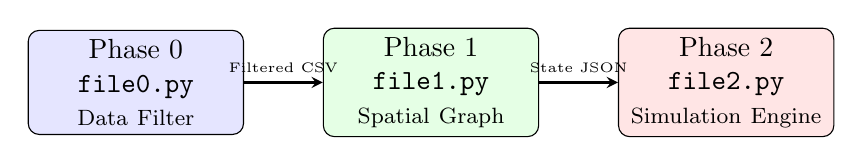
\begin{tikzpicture}[node distance=1cm]
    \node (p0) [block, fill=blue!10, text width=2.5cm] {Phase 0\\ \texttt{file0.py}\\ \footnotesize Data Filter};
    \node (p1) [block, fill=green!10, right=of p0, text width=2.5cm] {Phase 1\\ \texttt{file1.py}\\ \footnotesize Spatial Graph};
    \node (p2) [block, fill=red!10, right=of p1, text width=2.5cm] {Phase 2\\ \texttt{file2.py}\\ \footnotesize Simulation Engine};
    
    \draw [arrow] (p0) -- (p1) node[midway, above, font=\tiny] {Filtered CSV};
    \draw [arrow] (p1) -- (p2) node[midway, above, font=\tiny] {State JSON};
  \end{tikzpicture}
  \end{center}
  \vspace{0.3cm}
  \begin{itemize}
      \item \textbf{Phase 0:} \texttt{file0.py} isolates chronologically sorted 1-hour Manhattan demand.
      \item \textbf{Phase 1:} \texttt{file1.py} flood-fills (Dijkstra) mapping GPS to feasible nodes.
      \item \textbf{Phase 2:} \texttt{file2.py} executes combinatorial dispatch and TraCI/SUMO physics.
  \end{itemize}
\end{frame}

\begin{frame}{File 0: Data Extraction \& Filtering}
  \textbf{Objective:} Create a clean, memory-safe, and highly localized demand dataset.
  \vspace{0.2cm}
  
  \begin{center}
  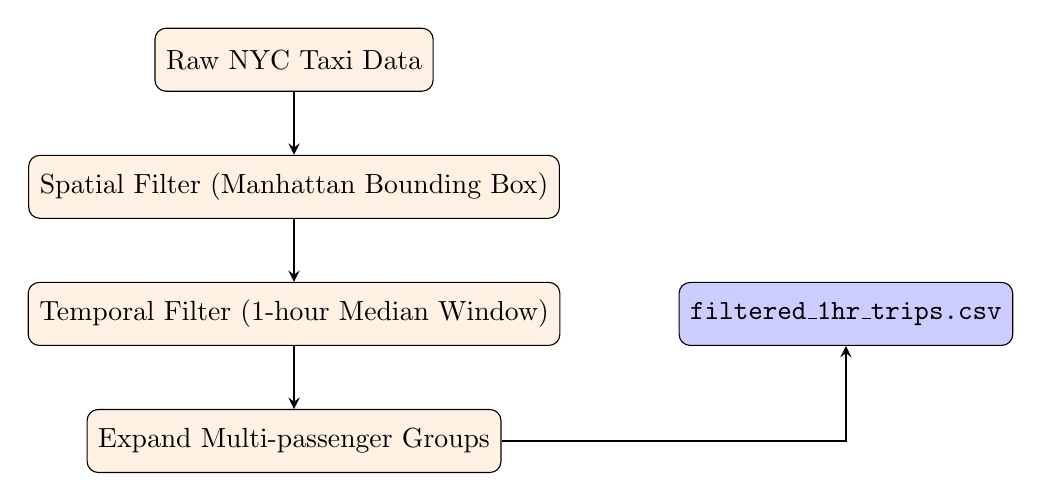
\begin{tikzpicture}[node distance=0.8cm]
    \node (raw) [process] {Raw NYC Taxi Data};
    \node (spatial) [process, below=of raw] {Spatial Filter (Manhattan Bounding Box)};
    \node (temporal) [process, below=of spatial] {Temporal Filter (1-hour Median Window)};
    \node (expand) [process, below=of temporal] {Expand Multi-passenger Groups};
    \node (out) [process, fill=blue!20, right=1.5cm of temporal] {\texttt{filtered\_1hr\_trips.csv}};
    
    \draw [arrow] (raw) -- (spatial);
    \draw [arrow] (spatial) -- (temporal);
    \draw [arrow] (temporal) -- (expand);
    \draw [arrow] (expand.east) -| (out.south);
  \end{tikzpicture}
  \end{center}
\end{frame}

\begin{frame}{File 1: Spatial Translation \& Graph Algorithms}
  \textbf{Objective:} Map arbitrary geographic coordinates to valid physical road network edges and calculate walking distances.
  \vspace{0.2cm}
  
  \begin{columns}
  \column{0.5\textwidth}
  \begin{center}
  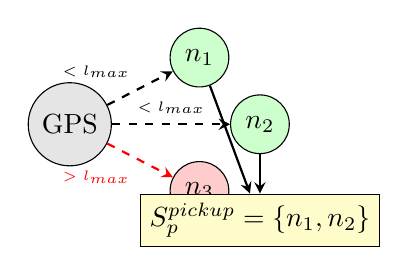
\begin{tikzpicture}[node distance=1.2cm]
    \node (gps) [circle, draw=black, fill=gray!20] {GPS};
    \node (n1) [circle, draw=black, fill=green!20, above right=0.2cm and 1cm of gps] {$n_1$};
    \node (n2) [circle, draw=black, fill=green!20, right=1.5cm of gps] {$n_2$};
    \node (n3) [circle, draw=black, fill=red!20, below right=0.2cm and 1cm of gps] {$n_3$};
    
    \draw [arrow, dashed] (gps) -- (n1) node[midway, above left, font=\tiny] {$< l_{max}$};
    \draw [arrow, dashed] (gps) -- (n2) node[midway, above, font=\tiny] {$< l_{max}$};
    \draw [arrow, dashed, red] (gps) -- (n3) node[midway, below left, font=\tiny] {$> l_{max}$};
    
    \node (set) [rectangle, draw=black, fill=yellow!20, below=0.5cm of n2] {$S^{pickup}_p = \{n_1, n_2\}$};
    \draw [arrow] (n1) -- (set);
    \draw [arrow] (n2) -- (set);
  \end{tikzpicture}
  \end{center}
  
  \column{0.5\textwidth}
  \begin{itemize}
      \item \textbf{Network Ingestion:} Loads \texttt{manhattan\_clean.net.xml}.
      \item \textbf{Dijkstra Flood-Fill:} Finds valid pickup nodes ($S^{pickup}_p$) and dropoff nodes ($S^{dropoff}_p$) reachable within max walking distance.
  \end{itemize}
  \end{columns}
\end{frame}

\begin{frame}{File 2: Detailed Execution Pipeline Overview}
  \begin{center}
  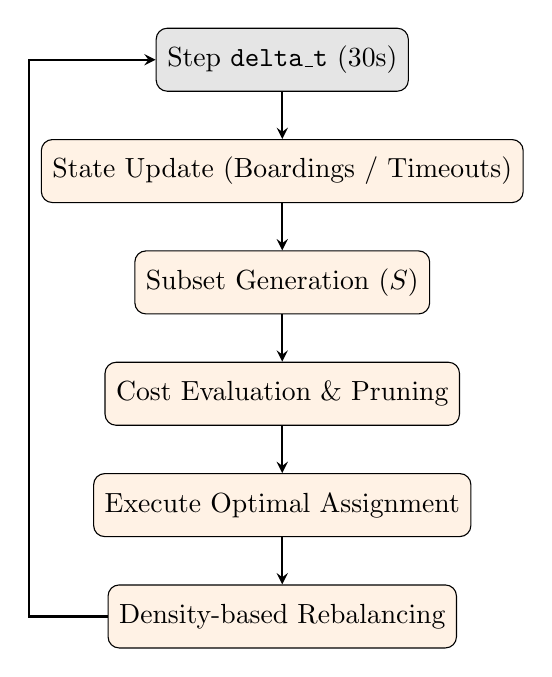
\begin{tikzpicture}[node distance=0.6cm]
    \node (start) [process, fill=gray!20] {Step \texttt{delta\_t} (30s)};
    \node (update) [process, below=of start] {State Update (Boardings / Timeouts)};
    \node (subset) [process, below=of update] {Subset Generation ($S$)};
    \node (eval) [process, below=of subset] {Cost Evaluation \& Pruning};
    \node (assign) [process, below=of eval] {Execute Optimal Assignment};
    \node (rebal) [process, below=of assign] {Density-based Rebalancing};
    
    \draw [arrow] (start) -- (update);
    \draw [arrow] (update) -- (subset);
    \draw [arrow] (subset) -- (eval);
    \draw [arrow] (eval) -- (assign);
    \draw [arrow] (assign) -- (rebal);
    \draw [arrow] (rebal.west) -- +(-1,0) |- (start.west);
  \end{tikzpicture}
  \end{center}
\end{frame}

\begin{frame}{File 2: Initialization \& Network Setup}
  \textbf{\texttt{load\_state()} \& \texttt{build\_network()}}
  \begin{itemize}
      \item Reads \texttt{simulation\_state.json} generated by File 1.
      \item Uses \texttt{sumolib} to build an internal memory representation of \texttt{manhattan\_clean.net.xml}.
      \item Pre-calculates distance matrices and initializes spatial anchors for faster routing checks.
  \end{itemize}
  \vspace{0.3cm}
  \textbf{\texttt{start\_sumo()}}
  \begin{itemize}
      \item Initiates the TraCI connection to the SUMO binary.
      \item Spawns the physical 3,000-vehicle fleet onto the network edges, ensuring they do not immediately despawn by appending safe "tail edges".
  \end{itemize}
\end{frame}

\begin{frame}{File 2: State Management \& Synchronization}
  \textbf{\texttt{detect\_pickups\_and\_dropoffs()}}
  \begin{itemize}
      \item Queries TraCI for every vehicle's physical edge ID.
      \item If a vehicle is on the exact edge as an assigned passenger, it triggers a "Boarding" or "Dropoff" event, freeing up vehicle capacity ($Cap_v$).
  \end{itemize}
  \vspace{0.3cm}
  \textbf{\texttt{release\_stale\_assignments()}}
  \begin{itemize}
      \item Iterates through all waiting passengers.
      \item If $t_{current} - t_{request} > W_{max}$ (10 minutes), the passenger is marked as a \textbf{Rejection} (Timeout) and purged from the queue.
      \item Frees vehicles that were assigned to passengers who gave up waiting.
  \end{itemize}
\end{frame}

\begin{frame}{File 2: Combinatorial Dispatch Engine (Part 1)}
  \textbf{\texttt{sample\_subsets()}}
  \begin{itemize}
      \item To prevent $O(N!)$ combinatorial explosions, this function groups nearby passengers into small sub-pools based on geographical proximity and time windows.
  \end{itemize}
  \vspace{0.3cm}
  \textbf{\texttt{evaluate\_subset()}}
  \begin{itemize}
      \item The mathematical core of the simulation. Tests every permutation of pickups and dropoffs for a subset of passengers.
      \item Returns the minimum possible Objective Cost for that specific subset.
  \end{itemize}
\end{frame}

\begin{frame}{File 2: Combinatorial Dispatch Engine (Part 2)}
  \textbf{The Pruning Mechanism inside \texttt{evaluate\_subset()}:}
  \begin{center}
  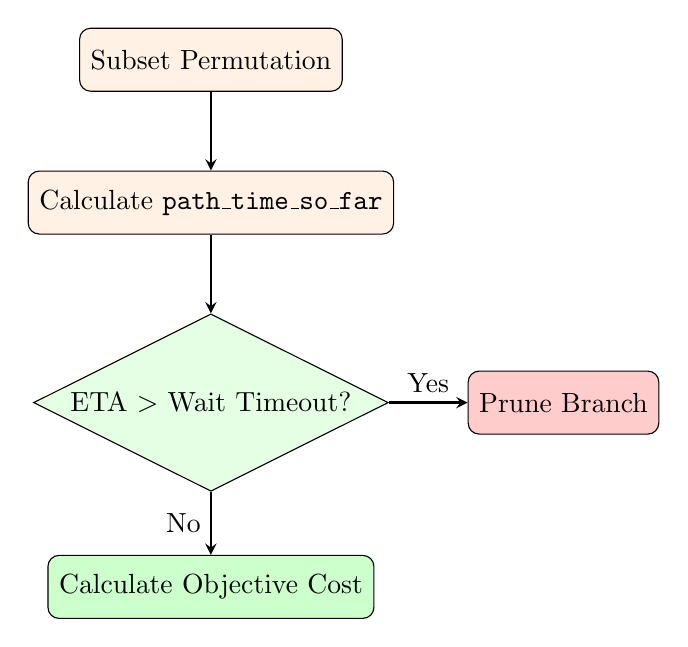
\begin{tikzpicture}[node distance=1cm]
    \node (root) [process] {Subset Permutation};
    \node (calc) [process, below=of root] {Calculate \texttt{path\_time\_so\_far}};
    \node (dec) [decision, below=of calc] {ETA $>$ Wait Timeout?};
    \node (prune) [process, fill=red!20, right=1cm of dec] {Prune Branch};
    \node (cost) [process, fill=green!20, below=0.8cm of dec] {Calculate Objective Cost};
    
    \draw [arrow] (root) -- (calc);
    \draw [arrow] (calc) -- (dec);
    \draw [arrow] (dec) -- node[anchor=south] {Yes} (prune);
    \draw [arrow] (dec) -- node[anchor=east] {No} (cost);
  \end{tikzpicture}
  \end{center}
  \vspace{0.2cm}
  \footnotesize
  \textbf{Crucial Check:} Tracking \texttt{path\_time\_so\_far} mathematically prevents the "starvation" bug where assigned passengers time out while waiting for a detouring vehicle.
\end{frame}

\begin{frame}{File 2: Cost Function}
  \textbf{The Objective Cost Function (\texttt{evaluate\_subset}):}
  \vspace{0.2cm}
  
  \[ Cost = \underbrace{\gamma(\Delta_v)}_{\text{Detour}} + \underbrace{\alpha(d_{walk})}_{\text{Walking}} + \underbrace{\beta \sum (\overbrace{t_{in\_veh} - t_{ideal}}^{\text{Ride Delay}} + \overbrace{t_{wait}}^{\text{Wait Delay}})}_{\text{Total Passenger Penalty}} + \underbrace{\mu(Cap_v - |S|)}_{\text{Empty Seats}} \]
  
  \vspace{0.4cm}
  \begin{itemize}
      \item By adding $t_{wait}$ to the $\beta$ term, the algorithm actively minimizes passenger starvation.
      \item $\mu$ encourages high-capacity ride-sharing subsets over single-rider trips.
  \end{itemize}
\end{frame}

\begin{frame}{File 2: Assignment \& Routing Execution}
  \textbf{\texttt{choose\_best\_assignments()}}
  \begin{itemize}
      \item Takes the cheapest evaluated subsets and greedily assigns them to the physical vehicles.
      \item Resolves conflicts where multiple vehicles want the same passenger.
  \end{itemize}
  \vspace{0.3cm}
  \textbf{\texttt{\_route\_vehicle\_to\_pending\_stops()} \& \texttt{set\_vehicle\_route()}}
  \begin{itemize}
      \item Translates the logical assignment array into physical SUMO waypoints.
      \item Uses \texttt{traci.vehicle.changeTarget()} and \texttt{traci.vehicle.setVia()} to force the vehicle along the mathematically optimal path without SUMO re-routing it unexpectedly.
  \end{itemize}
\end{frame}

\begin{frame}{File 2: Dynamic Fleet Rebalancing}
  \textbf{\texttt{build\_idle\_vehicle\_grid()} \& \texttt{maybe\_extend\_vehicle()}:}
  \begin{columns}
  \column{0.4\textwidth}
  \begin{center}
  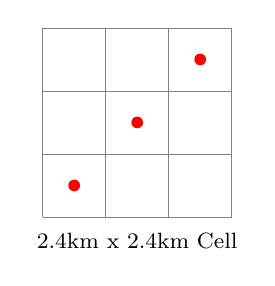
\begin{tikzpicture}
    \draw[step=0.8cm,gray,very thin] (0,0) grid (2.4,2.4);
    \node[circle, fill=red, inner sep=1.5pt] at (0.4, 0.4) {};
    \node[circle, fill=red, inner sep=1.5pt] at (1.2, 1.2) {};
    \node[circle, fill=red, inner sep=1.5pt] at (2.0, 2.0) {};
    \node at (1.2, -0.3) {\footnotesize 2.4km x 2.4km Cell};
  \end{tikzpicture}
  \end{center}
  
  \column{0.6\textwidth}
  \begin{itemize}
      \item Divides Manhattan into 2.4km grid cells and maps empty vehicles.
      \item \textbf{If Density $< 100$:} Vehicle parks (Saves deadheading cost).
      \item \textbf{If Density $\geq 100$:} Dispatched to historical demand hotspot.
  \end{itemize}
  \end{columns}
\end{frame}

\begin{frame}{File 2: Simulation Finalization}
  \textbf{\texttt{run\_cooldown\_phase()}}
  \begin{itemize}
      \item Executes after the 1-hour demand window closes.
      \item Stops accepting new requests and allows active vehicles to naturally complete their remaining dropoffs.
  \end{itemize}
  \vspace{0.3cm}
  \textbf{\texttt{write\_summary\_md()}}
  \begin{itemize}
      \item Aggregates all global metrics (Total Cost, Rejection Rate, Average Detour, Deadheading Ratio).
      \item Generates the final \texttt{analysis\_simulation\_trace.md} report used to evaluate the Alonso-Mora benchmark progress.
  \end{itemize}
\end{frame}

\begin{frame}{Alonso-Mora Algorithm: Core Methodology}
  \textbf{Background:} The 2017 paper by Alonso-Mora et al. introduced a highly scalable, anytime-optimal approach to assign groups of travelers.
  
  \begin{center}
  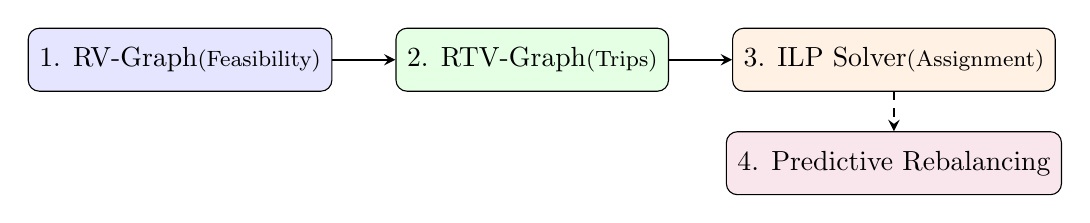
\begin{tikzpicture}[node distance=0.8cm]
    \node (rv) [process, fill=blue!10] {1. RV-Graph\\ \footnotesize (Feasibility)};
    \node (rtv) [process, fill=green!10, right=of rv] {2. RTV-Graph\\ \footnotesize (Trips)};
    \node (ilp) [process, fill=orange!10, right=of rtv] {3. ILP Solver\\ \footnotesize (Assignment)};
    \node (reb) [process, fill=purple!10, below=0.5cm of ilp] {4. Predictive Rebalancing};
    
    \draw [arrow] (rv) -- (rtv);
    \draw [arrow] (rtv) -- (ilp);
    \draw [arrow, dashed] (ilp) -- (reb);
  \end{tikzpicture}
  \end{center}
\end{frame}

\begin{frame}{Alonso-Mora Step 1: The Request-Vehicle (RV) Graph}
  \textbf{Objective:} Quickly filter out impossible passenger combinations before doing heavy routing calculations.
  
  \begin{columns}
  \column{0.5\textwidth}
  \begin{center}
  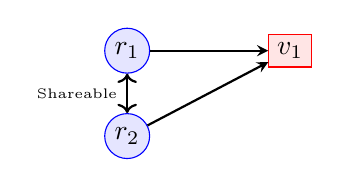
\begin{tikzpicture}[node distance=1.5cm]
    \node[circle, draw=blue, fill=blue!10, inner sep=2pt] (r1) {$r_1$};
    \node[circle, draw=blue, fill=blue!10, inner sep=2pt, below=0.5cm of r1] (r2) {$r_2$};
    \node[rectangle, draw=red, fill=red!10, inner sep=3pt, right=1.5cm of r1] (v1) {$v_1$};
    
    \draw[thick, <->] (r1) -- (r2) node[midway, left, font=\tiny] {Shareable};
    \draw[arrow] (r1) -- (v1);
    \draw[arrow] (r2) -- (v1);
  \end{tikzpicture}
  \end{center}
  \column{0.5\textwidth}
  \begin{itemize}
      \item Computes pairwise shareability. 
      \item Two requests share an edge if they can be served together without violating max wait time or delay constraints.
      \item \textbf{Result:} A bipartite graph connecting Requests to Vehicles.
  \end{itemize}
  \end{columns}
\end{frame}

\begin{frame}{Alonso-Mora Step 2: The Request-Trip-Vehicle (RTV) Graph}
  \textbf{Objective:} Generate all valid "Trips" (a combination of multiple requests served by one vehicle).
  \vspace{0.2cm}
  
  \begin{columns}
  \column{0.5\textwidth}
  \begin{center}
  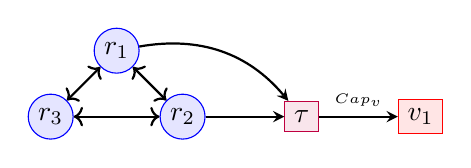
\begin{tikzpicture}[node distance=1cm]
    \node[circle, draw=blue, fill=blue!10, inner sep=2pt] (r1) {$r_1$};
    \node[circle, draw=blue, fill=blue!10, inner sep=2pt, below right=0.6cm of r1] (r2) {$r_2$};
    \node[circle, draw=blue, fill=blue!10, inner sep=2pt, below left=0.6cm of r1] (r3) {$r_3$};
    \draw[thick, <->] (r1) -- (r2); \draw[thick, <->] (r2) -- (r3); \draw[thick, <->] (r3) -- (r1);
    
    \node[rectangle, draw=purple, fill=purple!10, right=1cm of r2] (t1) {$\tau$};
    \node[rectangle, draw=red, fill=red!10, right=1cm of t1] (v1) {$v_1$};
    
    \draw[arrow] (r1) edge[bend left] (t1);
    \draw[arrow] (r2) -- (t1);
    \draw[arrow] (t1) -- (v1) node[midway, above, font=\tiny] {$Cap_v$};
  \end{tikzpicture}
  \end{center}
  \column{0.5\textwidth}
  \begin{itemize}
      \item Explores \textbf{cliques} (fully connected subgraphs) within the RV-graph.
      \item Verifies if a specific vehicle $v$ can execute trip $\tau$ while respecting capacity ($Cap_v$).
  \end{itemize}
  \end{columns}
\end{frame}

\begin{frame}{Alonso-Mora Step 3: Integer Linear Programming (ILP)}
  \textbf{Objective:} Find the single, globally optimal assignment of vehicles to trips. \\
  \textbf{Formulation:} Let $x_{\tau,v} \in \{0, 1\}$ represent whether vehicle $v$ is assigned to trip $\tau$.
  \vspace{0.2cm}
  
  \begin{center}
  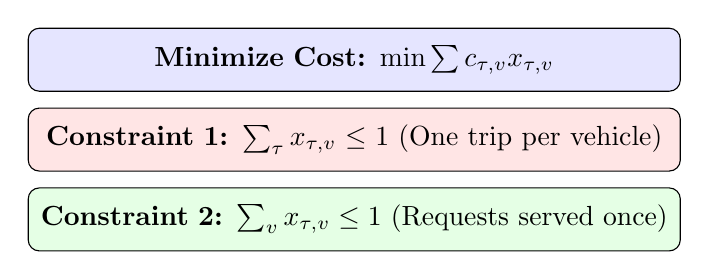
\begin{tikzpicture}
    \node (obj) [process, fill=blue!10, text width=8cm] {\textbf{Minimize Cost:} $ \min \sum c_{\tau,v} x_{\tau,v} $};
    \node (c1) [process, fill=red!10, below=0.2cm of obj, text width=8cm] {\textbf{Constraint 1:} $\sum_{\tau} x_{\tau,v} \leq 1$ (One trip per vehicle)};
    \node (c2) [process, fill=green!10, below=0.2cm of c1, text width=8cm] {\textbf{Constraint 2:} $\sum_{v} x_{\tau,v} \leq 1$ (Requests served once)};
  \end{tikzpicture}
  \end{center}
  \vspace{0.3cm}
  \textbf{Anytime Optimality:} Because solving large ILPs is NP-hard, the algorithm starts with a fast greedy solution and improves it using branch-and-bound. If the 30-second window closes, it simply returns the best valid assignment found so far.
\end{frame}

\begin{frame}{Results: Benchmark vs. Current Simulation Engine}
  \textbf{Scenario Details:} 3,000 vehicles, capacity 4, 1-hour NYC Taxi Demand.
  \vspace{0.3cm}
  
  \begin{table}[]
      \centering
      \begin{tabular}{|l|c|c|}
      \hline
      \textbf{Metric} & \textbf{Alonso-Mora (2017)} & \textbf{Our Engine (v2.0)} \\ \hline
      \textbf{Service Rate} & $\sim 98.0\%$ & \textbf{94.5\%} \\ \hline
      \textbf{Rejection Rate} & $\sim 2.0\%$ & 4.8\% \\ \hline
      \textbf{Mean Waiting Time} & 2.7 minutes (162s) & \textbf{15.2 seconds} \\ \hline
      \textbf{Mean Delay/Detour} & 2.3 minutes (138s) & $\sim 0$ seconds (0.89x) \\ \hline
      \end{tabular}
  \end{table}
  \vspace{0.1cm}
  \footnotesize{*Our actual travel time (315.7s) is less than the ideal vehicle path (354.0s) because passengers walked an average of 99.8m to optimal pickup nodes.}
\end{frame}

\begin{frame}{Analysis of Results \& Discrepancies}
  \textbf{Why is our Service Rate slightly lower (94.5\% vs 98\%)?}
  \begin{itemize}
      \item \textbf{Greedy vs. ILP:} While Alonso-Mora uses an Integer Linear Program to find the global optimum across all trips simultaneously, our current engine uses a reactive, localized combinatorial search (\texttt{evaluate\_subset}). We occasionally make sub-optimal regional assignments that leave other passengers starved.
      \item \textbf{Reactive vs. Predictive Rebalancing:} Our 4.8\% rejections are entirely due to 10-minute timeouts. Our empty vehicles currently rebalance \textit{reactively} (moving to historical hotspots only after a zone becomes too crowded). Alonso-Mora uses \textit{predictive} routing to pre-position vehicles before demand strikes.
  \end{itemize}
\end{frame}

\begin{frame}{Analysis of Results: Waiting Time \& Fleet Efficiency}
  \textbf{Why is our Mean Waiting Time exponentially faster (15s vs 162s)?}
  \begin{itemize}
      \item Our aggressive \texttt{MIN\_IDLE\_DENSITY} rebalancing floods the Manhattan grid with empty vehicles. When a request drops, there is almost always a vehicle on the same or adjacent edge.
      \item \textbf{The Trade-off:} This comes at the cost of a massive \textbf{86.6\% Deadheading Ratio}. Our vehicles spend the vast majority of their time driving empty in circles.
  \end{itemize}
\end{frame}

\begin{frame}{Conclusion \& Roadmap}
  \begin{center}
  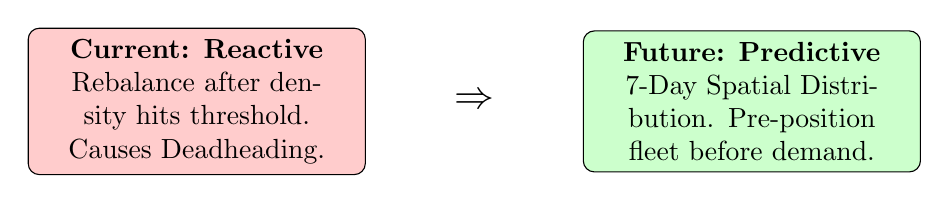
\begin{tikzpicture}
    \node (react) [process, fill=red!20, text width=4cm] {\textbf{Current: Reactive}\\ Rebalance after density hits threshold. Causes Deadheading.};
    \node (arrow) [right=of react] {\textbf{\Large $\Rightarrow$}};
    \node (predict) [process, fill=green!20, right=of arrow, text width=4cm] {\textbf{Future: Predictive}\\ 7-Day Spatial Distribution. Pre-position fleet before demand.};
  \end{tikzpicture}
  \end{center}
  \vspace{0.5cm}
  \textbf{Next Steps to hit 98\% Benchmark:}
  \begin{enumerate}
      \item Implement the \textbf{7-day Predictive Spatial Distribution Model} to eliminate deadheading and prevent localized starvation.
      \item Transition \texttt{evaluate\_subset} to a global optimization mechanism inspired by the Alonso-Mora ILP formulation.
  \end{enumerate}
\end{frame}

\end{document}
